\usetikzlibrary{positioning, arrows.meta, patterns}

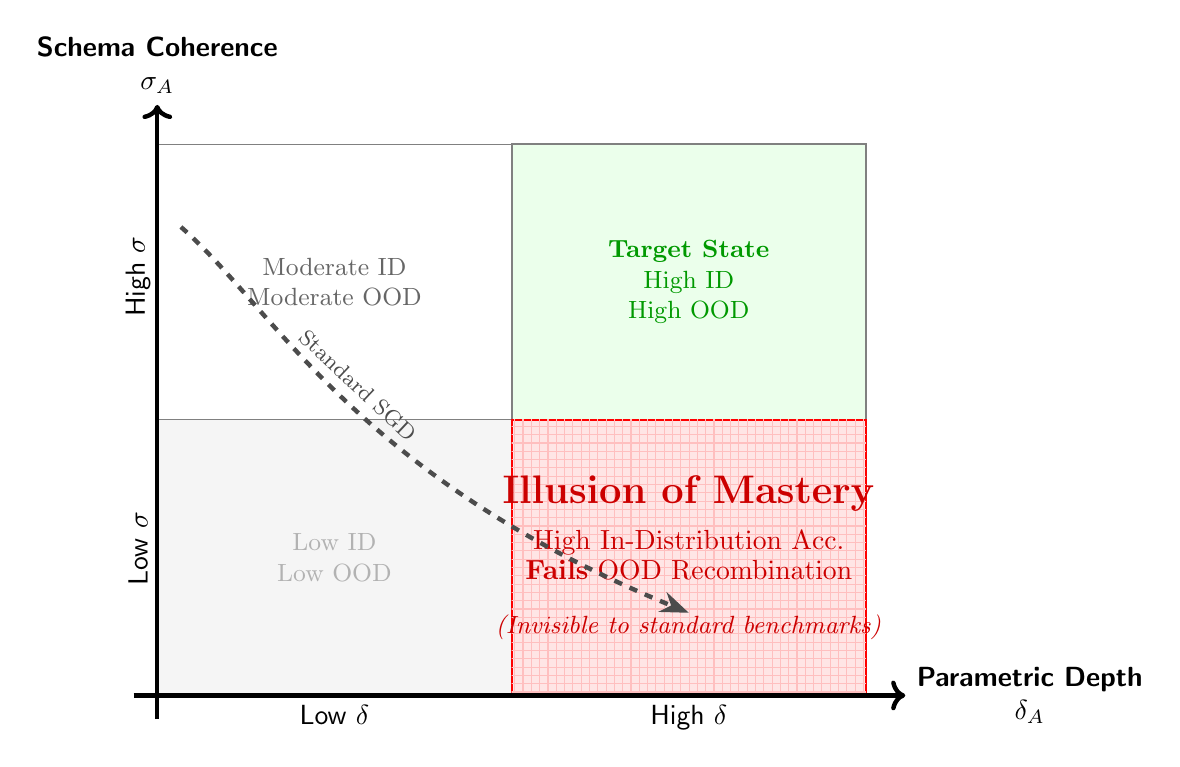
\begin{tikzpicture}[font=\sffamily]

    % Dimensions
    \def\w{4.5} % Width of quadrant
    \def\h{3.5} % Height of quadrant

    % Base Grid & Quadrants
    \filldraw[fill=white, draw=gray] (0, \h) rectangle (\w, 2*\h); % Top-Left
    \filldraw[fill=green!8, draw=gray, thick] (\w, \h) rectangle (2*\w, 2*\h); % Top-Right (Target)
    \filldraw[fill=gray!8, draw=gray] (0, 0) rectangle (\w, \h); % Bottom-Left

    % The Diagnostic Cell (Bottom-Right) with grid pattern for grayscale
    \filldraw[fill=red!10, draw=red, thick] (\w, 0) rectangle (2*\w, \h);
    \fill[pattern=grid, pattern color=red!25] (\w, 0) rectangle (2*\w, \h);

    % Axes
    \draw[->, ultra thick, black] (-0.3, 0) -- (2*\w + 0.5, 0) node[right, align=center] {\textbf{Parametric Depth}\\ $\delta_A$};
    \draw[->, ultra thick, black] (0, -0.3) -- (0, 2*\h + 0.5) node[above, align=center] {\textbf{Schema Coherence}\\ $\sigma_A$};

    % Axis Labels
    \node[below] at (\w/2, 0) {Low $\delta$};
    \node[below] at (\w*1.5, 0) {High $\delta$};
    \node[left, rotate=90, yshift=7pt, xshift=20pt] at (0, \h/2) {Low $\sigma$};
    \node[left, rotate=90, yshift=7pt, xshift=20pt] at (0, \h*1.5) {High $\sigma$};

    % Quadrant Text
    \node[align=center, text=gray!80!black, font=\small] at (\w/2, \h*1.5) {Moderate ID \\ Moderate OOD};
    \node[align=center, text=green!60!black, font=\small] at (\w*1.5, \h*1.5) {\textbf{Target State} \\ High ID \\ High OOD};
    \node[align=center, text=gray!60, font=\small] at (\w/2, \h/2) {Low ID \\ Low OOD};

    % Diagnostic Cell Text
    \node[align=center, text=red!80!black, font=\small] at (\w*1.5, \h/2) {
        \Large \textbf{Illusion of Mastery}\\[2mm]
        \normalsize High In-Distribution Acc.\\
        \normalsize \textbf{Fails} OOD Recombination\\[3mm]
        \small \textit{(Invisible to standard benchmarks)}
    };

    % Target symbol (checkmark in green quadrant)
    \node[font=\Large, text=green!70!black] at (\w*1.5, \h*1.5) [yshift=8mm, xshift=8mm] {$\bigstar$};

    % Danger symbol (warning in red quadrant)
    \node[font=\Large, text=red!70!black] at (\w*1.5, \h/2) [yshift=-6mm, xshift=-10mm] {$\blacksquare$};

    % Standard SGD trajectory arrow (black!70 for grayscale visibility)
    \draw[->, ultra thick, black!70, dashed, >=Stealth]
        (0.3, \h*1.7)
        .. controls (1.5, \h*1.4) and (2.5, \h*0.8) ..
        (\w*1.5, \h*0.3)
        node[midway, above, sloped, font=\footnotesize, text=black!70] {Standard SGD};

\end{tikzpicture}
